\problemname{Artwork}

A template for an artwork is a white grid of $n \times m$ squares.
The artwork will be created by painting $q$ horizontal and vertical black strokes.
A stroke starts from square $(x_1,y_1)$, ends at square $(x_2,y_2)$
($x_1=x_2$ or $y_1=y_2$) and changes the color of all squares $(x,y)$ to black
where $x_1 \le x \le x_2$ and $y_1 \le y \le y_2$.

The beauty of an artwork is the number of regions in the grid.
Each region consists of one or more white squares that are connected
to each other using a path of white squares in the grid, walking horizontally or vertically but not diagonally.
The initial beauty of the artwork is $1$. Your task is to calculate the
beauty after each new stroke.  Figure~\ref{fig:modern art sample} illustrates how the beauty of the artwork varies in Sample Input 1.

\begin{figure}[!h]
\centering
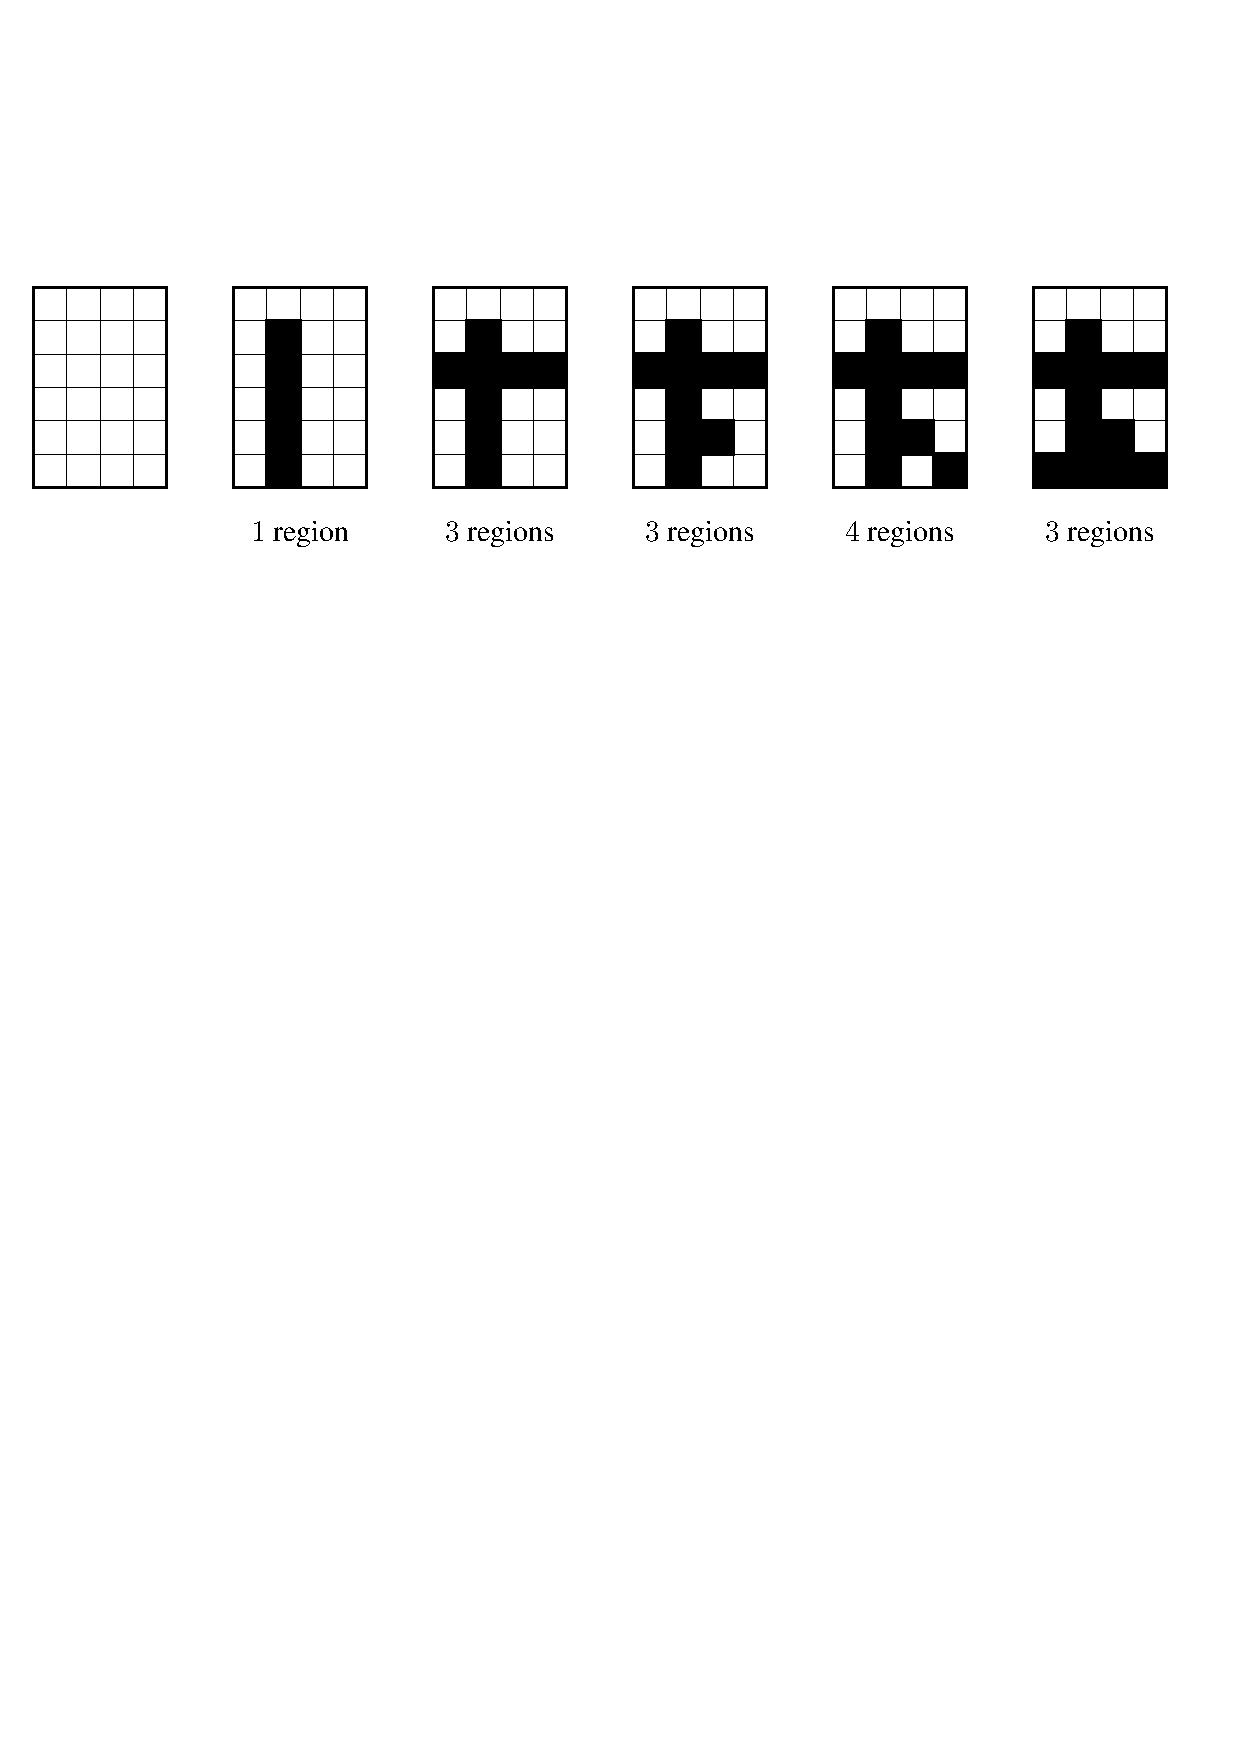
\includegraphics[width=0.9\textwidth]{sample}
\caption{Illustration of Sample Input 1.}
\label{fig:modern art sample}
\end{figure}

\section*{Input}

The first line of input contains three integers $n$, $m$ and $q$
($1 \le n,m \le 1000$, $1 \le q \le 10^4$).

Then follow $q$ lines that describe the strokes.
Each line consists of four integers $x_1$, $y_1$, $x_2$ and $y_2$
($1 \le x_1 \le x_2 \le n$, $1 \le y_1 \le y_2 \le m$).  Either $x_1 = x_2$ or $y_1 = y_2$ (or both).

\section*{Output}

For each of the $q$ strokes, output a line containing the beauty of the artwork after the stroke.
